\documentclass{llncs}
\usepackage{times}
\usepackage[T1]{fontenc}
\usepackage[utf8]{inputenc}

% Comentar para not MAC Users
%\usepackage[applemac]{inputenc}

\usepackage{a4}
%\usepackage[margin=3cm,nohead]{geometry}
\usepackage{epstopdf}
\usepackage{graphicx}
\usepackage{fancyvrb}
\usepackage{amsmath}
\usepackage{subcaption}
\usepackage[bookmarks=false]{hyperref}
%\renewcommand{\baselinestretch}{1.5}

\begin{document}
\mainmatter
\title{TP2: Protocolo IP}

\titlerunning{TP2: Protocolo IP}

\author{Diogo Afonso Costa \and Daniel Maia \and Vitor Castro}

\authorrunning{Diogo Afonso Costa \and Daniel Maia \and Vitor Castro}


\institute{
University of Minho, Department of  Informatics, 4710-057 Braga, Portugal\\
e-mail: \{a78034,a77531,a77870\}@alunos.uminho.pt
}

\date{}
\bibliographystyle{splncs}

\maketitle
\section{Introdução}
Temos que fazer...

\section{Parte I - Datagramas e Fragmentação}

\subsection{Exercício 1.b.}
\subsubsection{Questão}\rule[-10pt]{0pt}{10pt}\\

Registe e analise o tráfego ICMP enviado por n1 e o tráfego ICMP recebido como resposta. Comente os resultados face ao comportamento esperado.

\subsubsection{Resposta}\rule[-10pt]{0pt}{10pt}\\

Inicialmente, é feito o envio de um pacote com o TTL = 1, que não recebe resposta porque \textit{time exceeded message}, que acontece quando um datagrama chega a um \textit{gateway} com TTL = 0 (será neste ponto que será enviada uma resposta para a fonte do pacote, notificando da situação). Então, o TTL é progressivamente incrementado até ser igual a 3, sendo que aí já recebe mensagem de resposta. É também possíver verificar que há envio de vários pacotes com o TTL = 1 e TTL = 2, prevenindo a perda de um pacote ou uma falha no sistema, atuando assim como uma redundância. Depois vemos que a partir que o TTL = 3 o TTL é incrementado a TTL= 8 e as replies são feitas com TTL = 62 constantemente, por definição.

O tamanho do pacote é 74 bytes mas a mensagem tem 60 bytes de tamanho sendo que 14 bytes são para o header do nível 2. Nesta mensagem de 60 bytes estão incluídos 20 bytes de header length (variáveis de acordo com o protocolo IPv4) e nos 40 bytes restantes temos o ICMP header (8 bytes) e ICMP payload (32 bytes), sendo Data resultante de 32 bytes. Vemos que a mensagem de 32 bytes aumentou em 42 bytes até o nível 2 de rede.

\subsubsection{Realização}\rule[-10pt]{0pt}{10pt}\\
\begin{figure}
	\begin{center}
	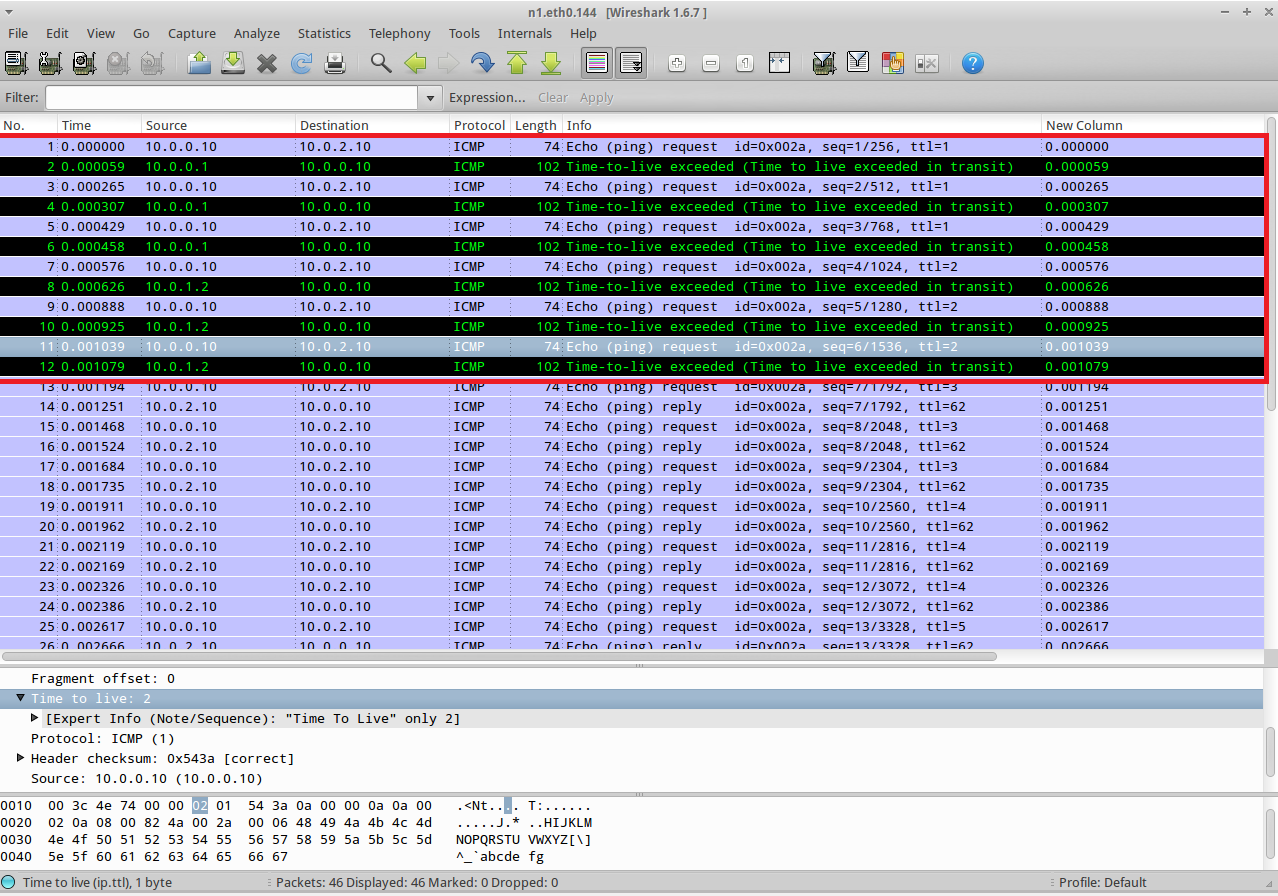
\includegraphics[scale=0.35]{imagens/ttlexceeded.png} 
	\end{center}
	\caption{\label{fig:ip_source}TTL excedido.}
\end{figure} 

\begin{figure}
	\begin{center}
	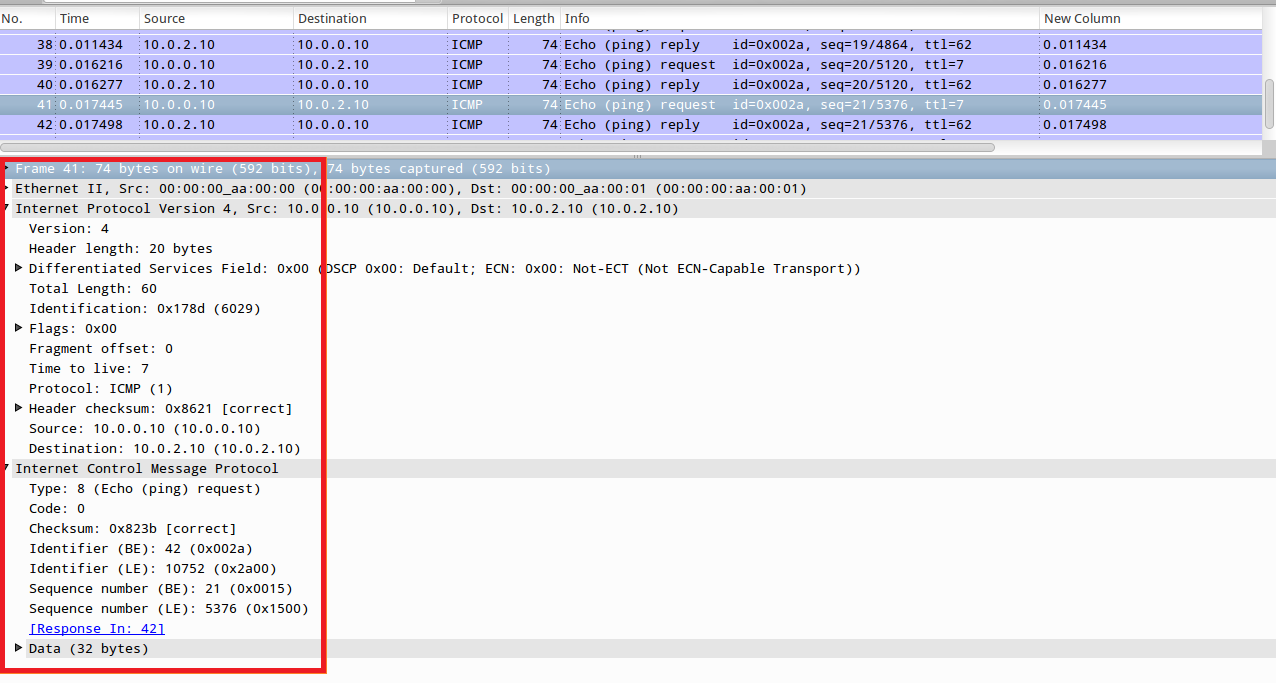
\includegraphics[scale=0.35]{imagens/bytesdata.png} 
	\end{center}
	\caption{\label{fig:ip_source}Tamanho do pacote e divisão.}
\end{figure} 

\subsection{Exercício 1.c.}
\subsubsection{Questão}\rule[-10pt]{0pt}{10pt}\\

Qual deve ser o valor inicial mínimo do campo TTL para alcançar o destino n4? Verifique na prática que a sua resposta está correta.

\subsubsection{Resposta}\rule[-10pt]{0pt}{10pt}\\

O TTL mínimo necessário para alcançar o destino n4 é 3. Isto é confirmado pelo \textit{wireshark}, que mostra que as tentativas com TTL menor que 3 resultou em \textit{time exceeded message}.

\subsubsection{Realização}\rule[-10pt]{0pt}{10pt}\\
\begin{figure}
	\begin{center}
	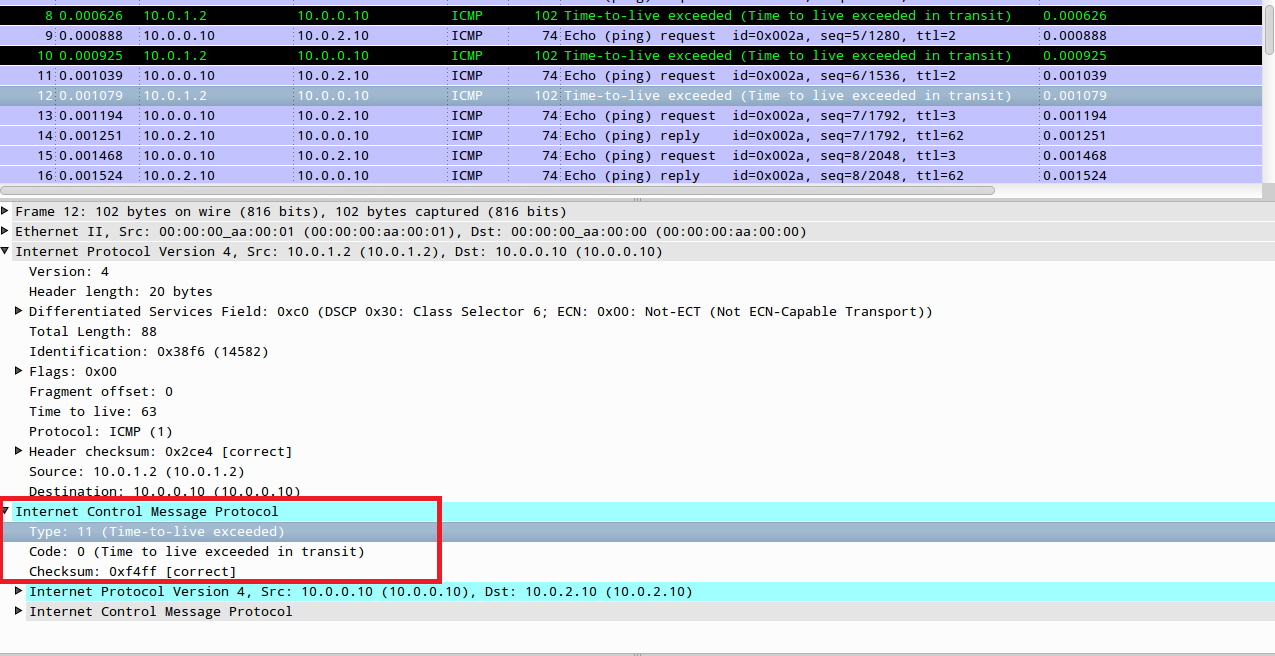
\includegraphics[scale=0.35]{imagens/ttlexceededmessage.png} 
	\end{center}
	\caption{\label{fig:ip_source}Mensagem com ICMP retornando TLL excedido.}
\end{figure} 

\subsection{Exercício 1.d.}
\subsubsection{Questão}\rule[-10pt]{0pt}{10pt}\\

Qual o valor médio do tempo de ida-e-volta (Round-Trip Time) obtido?

\subsubsection{Resposta}\rule[-10pt]{0pt}{10pt}\\

O Round-Trip Time é igual à soma do tempo de envio com o tempo de resposta. Logo, fazendo a soma das médias dos tempos, temos um resultado de Round-Trip Time médio de 0.00015 s (tempo de ida/request) + 0.00005 s (tempo de volta/reply) = 0.00020 s. É de notar que tanto o tempo de request como o de reply se mantêm relativamente constantes. Também se pode analisar este tempo recorrendo ao tempo relativo entre duas mensagens da mesma source.

\subsubsection{Realização}\rule[-10pt]{0pt}{10pt}\\
\begin{figure}
	\begin{center}
	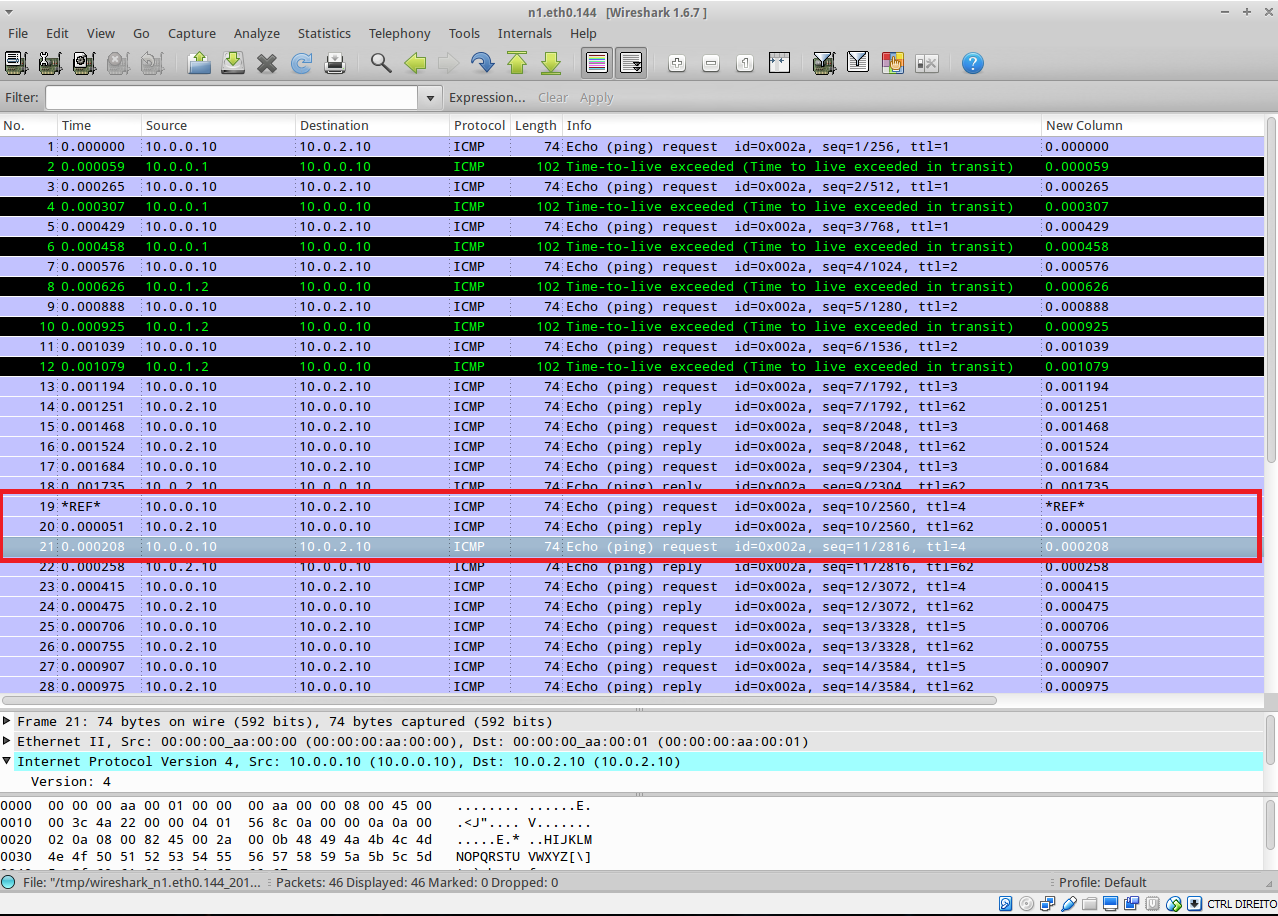
\includegraphics[scale=0.35]{imagens/roundtime.png} 
	\end{center}
	\caption{\label{fig:ip_source}Round-Trip Time.}
\end{figure} 

% Exercicio 2 --------------------

\subsection{Exercício 2.a.}
\subsubsection{Questão}\rule[-10pt]{0pt}{10pt}\\
Qual é o endereço IP da interface ativa do seu computador?

\subsubsection{Resposta}\rule[-10pt]{0pt}{10pt}\\
O endereço IP é 192.168.100.216. 

\subsubsection{Realização}\rule[-10pt]{0pt}{10pt}\\
\begin{figure}
	\begin{center}
	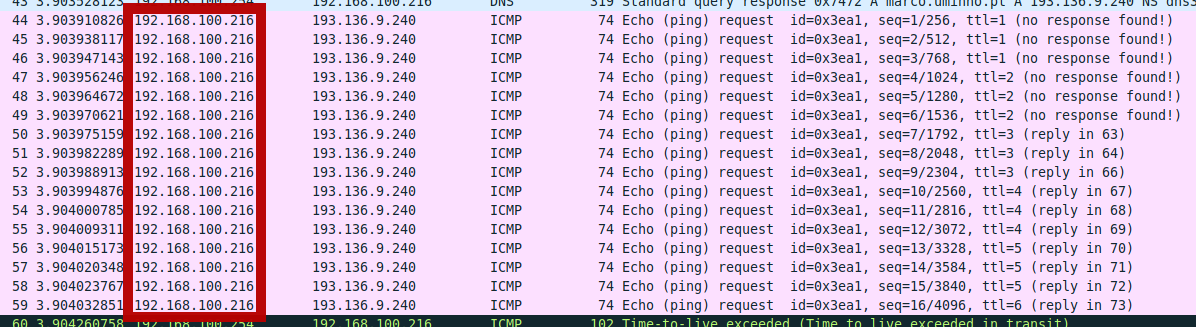
\includegraphics[scale=0.35]{imagens/ip_source_proof.png} 
	\end{center}
	\caption{\label{fig:ip_source}Identificação do endereço IP.}
\end{figure} 

% ------

\subsection{Exercício 2.b.}
\subsubsection{Questão}\rule[-10pt]{0pt}{10pt}\\

Qual é o valor do campo protocolo? O que identifica?

\subsubsection{Resposta}\rule[-10pt]{0pt}{10pt}\\

O campo protocolo tem o valor "ICMP (1)". ICMP significa \textit{Internet Control Message Protocol}. Este é utilizado para reportar erros no processamento de datagramas. Efetivamente, dentro dos possíveis erros temos, \textit{destination unreachable} (quando o datagrama não consegue alcançar o destino), \textit{time exceeded message} (quando um \textit{gateway} processa um datagrama e descobre que o \textit{TTL} é zero e tem que descartar o datagrama e consequentemente notificar o \textit{host}), \textit{echo request/reply} (quando são enviadas mensagens para funções de teste e controle da rede (\textit{request}), caso a máquina esteja ligada responde com um \textit{reply}) \cite{rfc792} \cite{wiki:ICMP_echo}. Como as mensagens ICMP encontram-se ao nível de rede, estas são também elas encapsuladas em datagramas IP que, consequentemente, usam o protocolo IP.

Assim sendo, analisando a primeira mensagem ICMP, nomeadamente no separador do \textit{Internet Protocol Version 4}, percebemos que se trata de uma mensagem que vem num protocolo \textit{ICMP}. Além disso, é possível concluir que se trata de uma mensagem de \textit{echo request}, se observarmos o campo \textit{Type} no separador \textit{Internet Control Message Protocol}. Desta forma, pode-se concluir que o computador usado para a resolução deste trabalho está a tentar perceber se consegue estabelecer uma ligação com o \textit{host} marco.uminho.pt e para isso usa mensagens \textit{ICMP} do tipo \textit{echo request}.

\subsubsection{Realização}\rule[-10pt]{0pt}{10pt}\\
\begin{figure}
	\begin{center}
	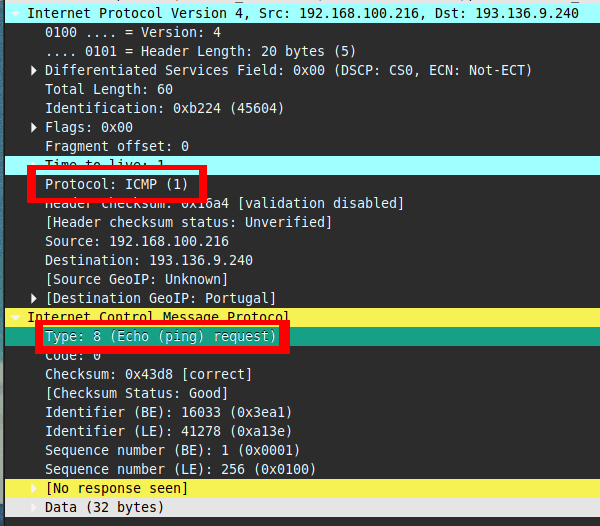
\includegraphics[scale=0.35]{./imagens/icmp_1.png} 
	\end{center}
	\caption{\label{fig:icmp_1}Identificação do campo \textit{Protocol}.}
\end{figure} 

% ------

\subsection{Exercício 2.c.}
\subsubsection{Questão}\rule[-10pt]{0pt}{10pt}\\

Quantos bytes tem o cabeçalho IP(v4)? Quantos bytes tem o campo de dados (payload) do datagrama? Como se calcula o tamanho do payload?  

\subsubsection{Resposta}\rule[-10pt]{0pt}{10pt}\\
	
O cabeçalho IPv4 tem 20 bytes.

O campo de dados (payload) do datagrama tem 40 bytes.

O cálculo do payload é feito retirando o tamanho do cabeçalho ao tamanho total do datagrama (60 bytes). Desta forma, basta fazer \(60 - 20 = 40 bytes\).

\subsubsection{Realização}\rule[-10pt]{0pt}{10pt}\\
\begin{figure}
	\begin{center}
	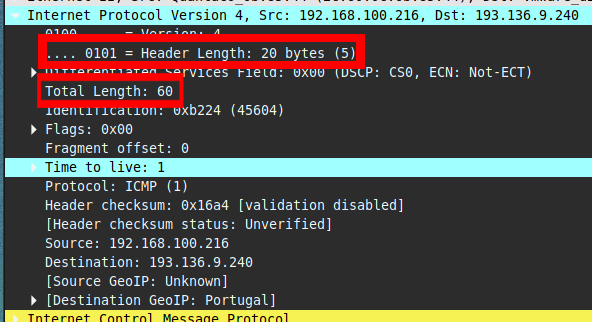
\includegraphics[scale=0.35]{./imagens/icmp_size.png} 
	\end{center}
	\caption{\label{fig:icmp_size}Identificação do tamanho do \textit{header} e do \textit{payload}.}
\end{figure} 

% ------

\subsection{Exercício 2.d.}
\subsubsection{Questão}\rule[-10pt]{0pt}{10pt}\\

O datagrama IP foi fragmentado? Justifique.

\subsubsection{Resposta}\rule[-10pt]{0pt}{10pt}\\

A fragmentação acontece quando o tamanho total do datagrama excede o \textit{MTU} disponível. Tendo em conta que por defeito o \textit{traceroute} usa 60 bytes por datagrama e tem-se um \textit{MTU} disponível de 1500 bytes, podemos conjeturar que não haverá fragmentação.
	
A verificação se um datagrama foi ou não fragmentado é feita com base em dois valores, o \textit{fragment offset} (indica o \textit{offset} em que o datagrama atual encaixa no datagrama original) e a \textit{flag more fragments} (indica se existe mais fragmentos). Neste datagrama em específico o \textit{fragment offset} = 0 e a \textit{flag more fragments} = 0. Desta forma, tendo em conta o \textit{fragment offset}, sabe-se que se o datagrama foi fragmentado então ele é necessariamente o primeiro. Além disso, se analisarmos a \textit{flag more fragments} concluímos que para além do datagrama atual não existe mais nenhum associado a este. 

Assim sendo, conjugando a informação dos dois parâmetros percebe-se que se o datagrama é o primeiro e não existe mais nenhum associado, então este é único e não foi fragmentado.

\subsubsection{Realização}\rule[-10pt]{0pt}{10pt}\\
\begin{figure}
	\begin{center}
	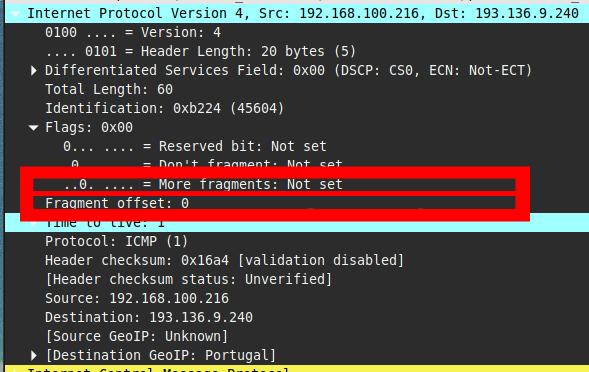
\includegraphics[scale=0.35]{./imagens/icmp_frag.png} 
	\end{center}
	\caption{\label{fig:icmp_frag}Fragmentação.}
\end{figure} 

% ------

\subsection{Exercício 2.e.}
\subsubsection{Questão}\rule[-10pt]{0pt}{10pt}\\

Ordene os pacotes capturados de acordo com o endereço IP fonte (e.g., selecionando o cabeçalho da coluna Source), e analise a sequência de tráfego ICMP gerado a partir do endereço IP atribuído à sua máquina. Para a sequência de mensagens ICMP enviadas pelo seu computador, indique que campos do cabeçalho IP variam de pacote para pacote.  

\subsubsection{Resposta}\rule[-10pt]{0pt}{10pt}\\

Os campos que vêm os seus valores alterados correspondem à \textit{identification}, \textit{header checksum} e \textit{time to live (TTL)}. 

A \emph{identificação} muda pois este campo identifica unicamente cada datagrama e visto que estes são sempre diferentes então o campo também o será.

O \textit{header checksum} permite verificar que determinado header foi ou não corrompido. Desta forma o \textit{checksum} identifica um determinado \textit{header} num determinado estado. Assim sendo, o \textit{checksum} muda pois este campo utiliza no seu algoritmo todas as palavras de 16 bits do \textit{header} \cite{rfc792}. Efetivamente, sabendo que o \textit{header}, propriamente dito, muda de datagrama para datagrama então o seu \textit{checksum} também vai mudar.

O \textit{TTL} muda pois a máquina que está a ser usada está a tentar contactar o \textit{host} marco.uminho.pt. Começa por tentar com \(TTL = 1\) e o pacote é descartado. Desta forma, vai aumentado o \textit{TTL} até conseguir chegar ao \textit{host} pretendido.

\subsubsection{Realização}\rule[-10pt]{0pt}{10pt}\\

\begin{figure}[h]
	\centering
	\begin{subfigure}{.4\textwidth}
		\centering
		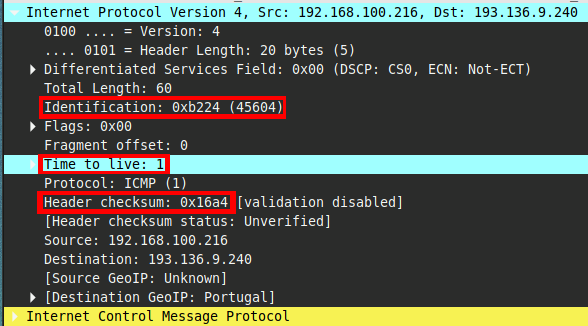
\includegraphics[width=0.98\linewidth]{./imagens/icmp_TTL_1.png}
	\end{subfigure}%
	\begin{subfigure}{.4\textwidth}
		\centering
		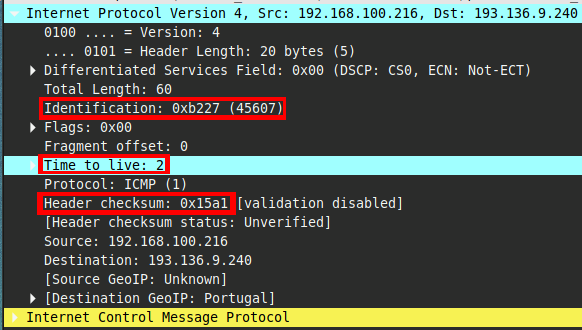
\includegraphics[width=0.98\linewidth]{./imagens/icmp_TTL_2.png}
	\end{subfigure}%
	\begin{subfigure}{.4\textwidth}
		\centering
		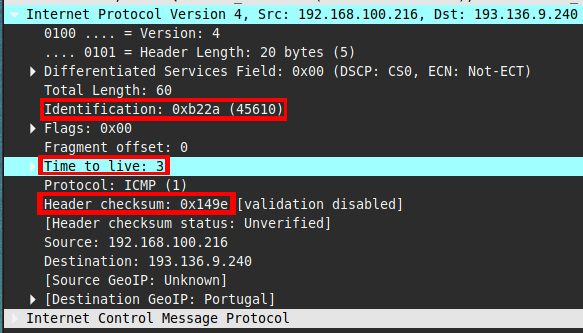
\includegraphics[width=0.98\linewidth]{./imagens/icmp_TTL_3.png}
	\end{subfigure}
	\caption{Campos que mudam.}
	\label{fig:field_change}
\end{figure}

% ------

\subsection{Exercício 2.f.}
\subsubsection{Questão}\rule[-10pt]{0pt}{10pt}\\

Observa algum padrão nos valores do campo de Identificação do datagrama IP e TTL? 

\subsubsection{Resposta}\rule[-10pt]{0pt}{10pt}\\

O campo da indentificação corresponde a um valor que é incrementado e que identifica unicamente o datagrama em questão. Por exemplo, se o primeiro datagrama tiver \textit{Identification} 0xb224 (45604), então o datagrama seguinte terá o valor 0xb225 (45605). 

O TTL corresponde a uma variável que vai sendo decrementada sempre que é intersetada por um \textit{router}. Visto que na primeira mensagem o TTL é 1, o datagrama é descartado imediatamente no primeiro \textit{router}. Deste modo, é enviado, de seguida, um novo datagrama com TTL a 2 com a esperança de que este chegue desta vez ao destino. Caso não chegue, então no próximo datagrama o TTL será aumentado, e assim sucessivamente, até chegar ao destino.

\subsubsection{Realização}\rule[-10pt]{0pt}{10pt}\\

A relação entre \textit{TTL} pode ser observada na figura ~\ref{fig:field_change}.

\begin{figure}[h]
	\centering
	\begin{subfigure}{.5\textwidth}
		\centering
		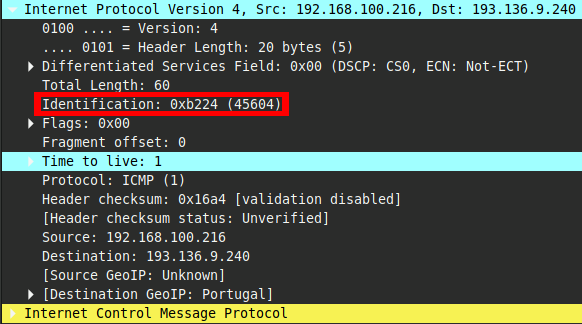
\includegraphics[width=0.98\linewidth]{./imagens/icmp_1_id.png}
	\end{subfigure}%
	\begin{subfigure}{.5\textwidth}
		\centering
		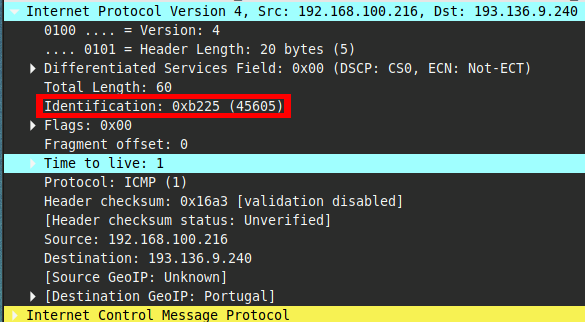
\includegraphics[width=0.98\linewidth]{./imagens/icmp_2_id.png}
	\end{subfigure}
	\caption{Identificação.}
	\label{fig:field_id}
\end{figure}

% ------

\subsection{Exercício 2.g.}
\subsubsection{Questão}\rule[-10pt]{0pt}{10pt}\\

Ordene o tráfego capturado por endereço destino e encontre a série de respostas ICMP TTL exceeded enviadas ao seu computador. Qual é o valor do campo TTL? Esse valor permanece constante para todas as mensagens de resposta ICMP TTL exceeded enviados ao seu host? Porquê? 

\subsubsection{Resposta}\rule[-10pt]{0pt}{10pt}\\

O IP 192.168.100.254 referencia a interface do primeiro router de acesso (visto ter o três primeiros campos iguais ao da máquina em que os testes estão a ser feitos e o último utiliza um número convencionado para ser utilizado para identificar a interface IP do router dentro da rede 192.168.100, na qual a máquina de testes se encontra).

Desta forma, quando analisamos os datagramas do 192.168.100.254 percebemos que estes têm todos o \textit{TTL} = 64. O \textit{TTL} toma um valor exageradamente elevado, devido ao desconhecimento que este tem da distância a que o \textit{host} de destino se encontra. Por defeito, este router quando não tem informação da distância a que o \textit{host} de destino se encontra envia datagramas com \textit{TTL} = 64 e por isso todas os seus datagramas tem \textit{TTL} igual.

Além disso, é possível concluir que as três mensagens recebidas deste router com \textit{ICMP \textit{TTL} exceeded} são a resposta ao envio feito pela máquina de testes de três datagramas de \textit{echo (ping) request} com \textit{TTL} apenas de 1. Estes datagramas chegaram ao \textit{router} de acesso e ficaram com o \textit{TTL} a 0 e a exceção veio enviado de no datagrama \textit{ICMP \textit{TTL} exceeded}.

Após estes datagramas é possível identificar um segundo conjunto de datagramas desta vez da interface IP 193.136.19.254. Pelo mesmo raciocínio podemos assumir que o IP desta interface identifica um \textit{router}. Este novo \textit{router} envia datagramas com \textit{TTL} = 254 (constante). Este valor é considerável pela mesma razão explicitada anteriormente. Estes datagramas são a resposta a 3 datagramas enviados pela máquina de testes com \textit{TTL} = 2, o que nos leva a concluir que é o segundo router por qual o nosso datagrama teve de passar para chegar ao marco.uminho.pt.

\subsubsection{Realização}\rule[-10pt]{0pt}{10pt}\\

\begin{figure}[h]
	\centering
	\begin{subfigure}{.4\textwidth}
		\centering
		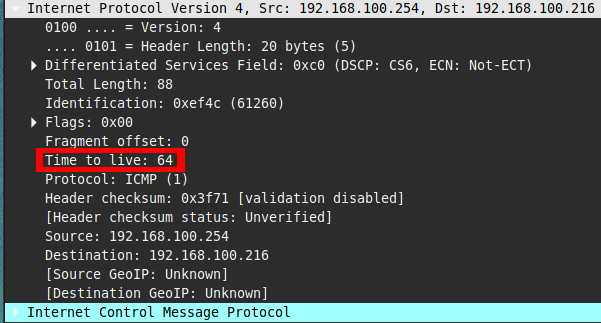
\includegraphics[width=0.98\linewidth]{./imagens/icmp_1_TTL64_router.png}
	\end{subfigure}%
	\begin{subfigure}{.4\textwidth}
		\centering
		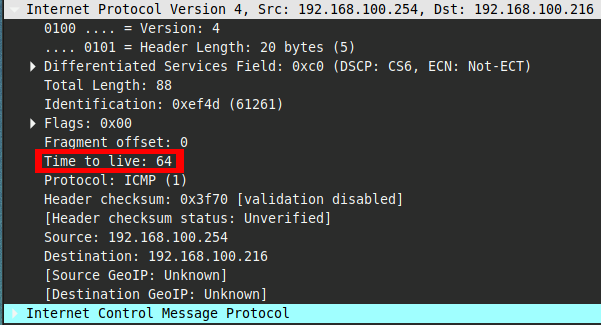
\includegraphics[width=0.98\linewidth]{./imagens/icmp_2_TTL64_router.png}
	\end{subfigure}%
	\begin{subfigure}{.4\textwidth}
		\centering
		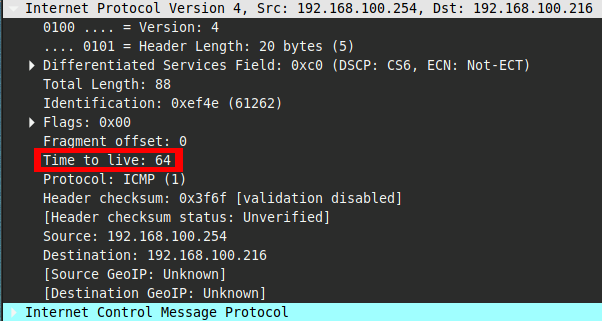
\includegraphics[width=0.98\linewidth]{./imagens/icmp_3_TTL64_router.png}
	\end{subfigure}
	\caption{Router de acesso com \textit{TTL} = 64.}
	\label{fig:field_change}
\end{figure}

\begin{figure}[h]
	\centering
	\begin{subfigure}{.4\textwidth}
		\centering
		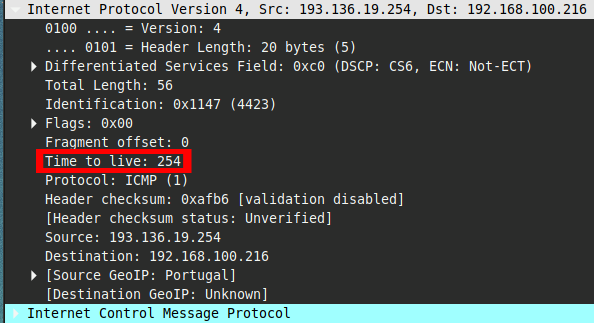
\includegraphics[width=0.98\linewidth]{./imagens/icmp_1_TTL254_router.png}
	\end{subfigure}%
	\begin{subfigure}{.4\textwidth}
		\centering
		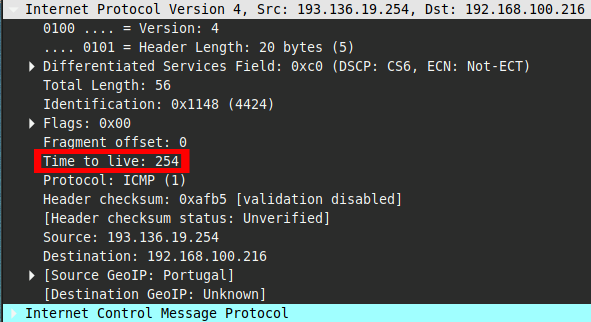
\includegraphics[width=0.98\linewidth]{./imagens/icmp_2_TTL254_router.png}
	\end{subfigure}%
	\begin{subfigure}{.4\textwidth}
		\centering
		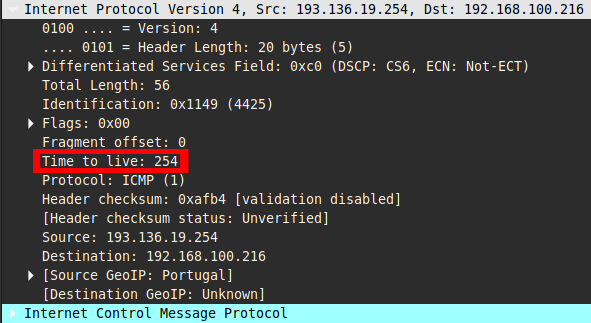
\includegraphics[width=0.98\linewidth]{./imagens/icmp_3_TTL254_router.png}
	\end{subfigure}
	\caption{Segundo router com \textit{TTL} = 254.}
	\label{fig:field_change}
\end{figure}

% Exercicio 3 --------------------

\subsection{Exercício 3.a.}
\subsubsection{Questão}\rule[-10pt]{0pt}{10pt}\\

Localize a primeira mensagem ICMP. Porque é que houve necessidade de fragmentar o pacote inicial?

\subsubsection{Resposta}\rule[-10pt]{0pt}{10pt}\\

O pacote inicial tem um \textit{total length} de 3033 bytes. O MTU (\textit{Maximum Transmission Unit} disponível é de apenas 1500 bytes e, como tal, o pacote inicial tem de ser fragmentado para que este possa ser transmitido na rede.

\subsubsection{Realização}\rule[-10pt]{0pt}{10pt}\\

\begin{figure}
	\begin{center}
	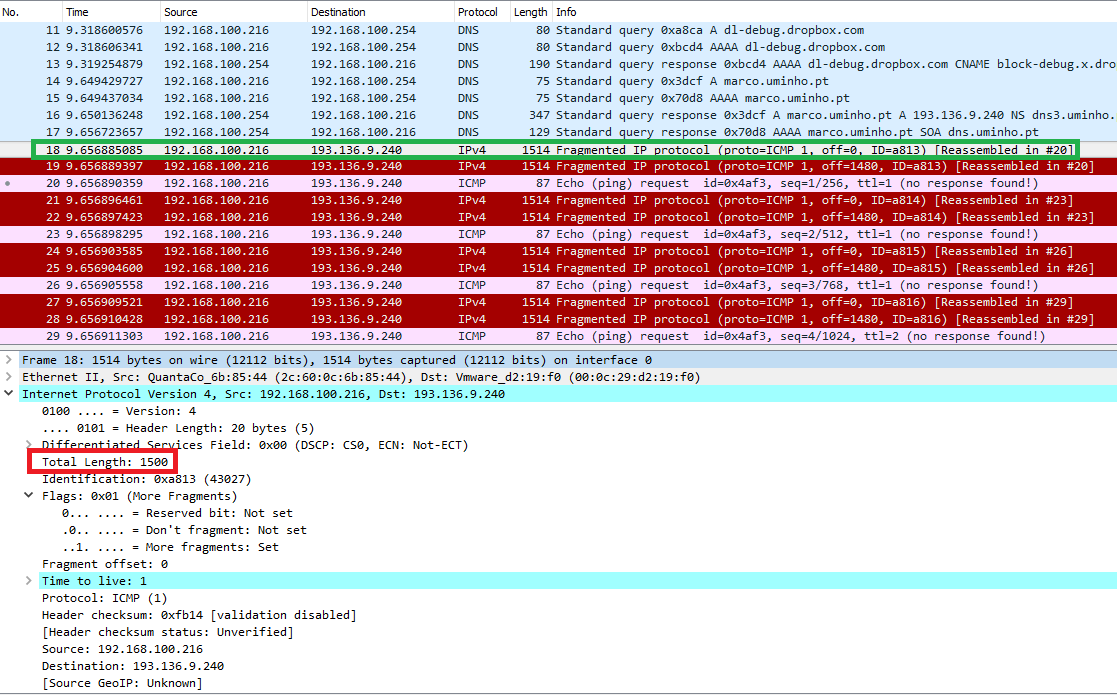
\includegraphics[scale=0.35]{./imagens/packet_frag.png} 
	\end{center}
	\caption{\label{fig:packet_frag}A MTU é menor do que o tamanho do pacote.}
\end{figure} 


\subsection{Exercício 3.b.}
\subsubsection{Questão}\rule[-10pt]{0pt}{10pt}\\

Imprima o primeiro fragmento do datagrama IP segmentado. Que informação no cabeçalho indica que o datagrama foi fragmentado? Que informação no cabeçalho IP indica que se trata do primeiro fragmento? Qual é o tamanho deste datagrama IP?

\subsubsection{Resposta}\rule[-10pt]{0pt}{10pt}\\

A informação de que o datagrama foi fragmentado é dada através da \textit{flag more fragments} que se encontra a 1 em conjugação com o campo \textit{fragment offset}, que neste caso se encontra a 0. Desta forma, podemos concluir que este datagrama é efetivamente o primeiro (\textit{fragment offset} = 0) de um PDU fragmentado (\textit{flag more fragments} = 1). Este é um datagrama IP de 1480 bytes (MTU de 1500 bytes, dos quais 20 bytes servem de \textit{header}). 

\subsubsection{Realização}\rule[-10pt]{0pt}{10pt}\\

\begin{figure}
	\begin{center}
	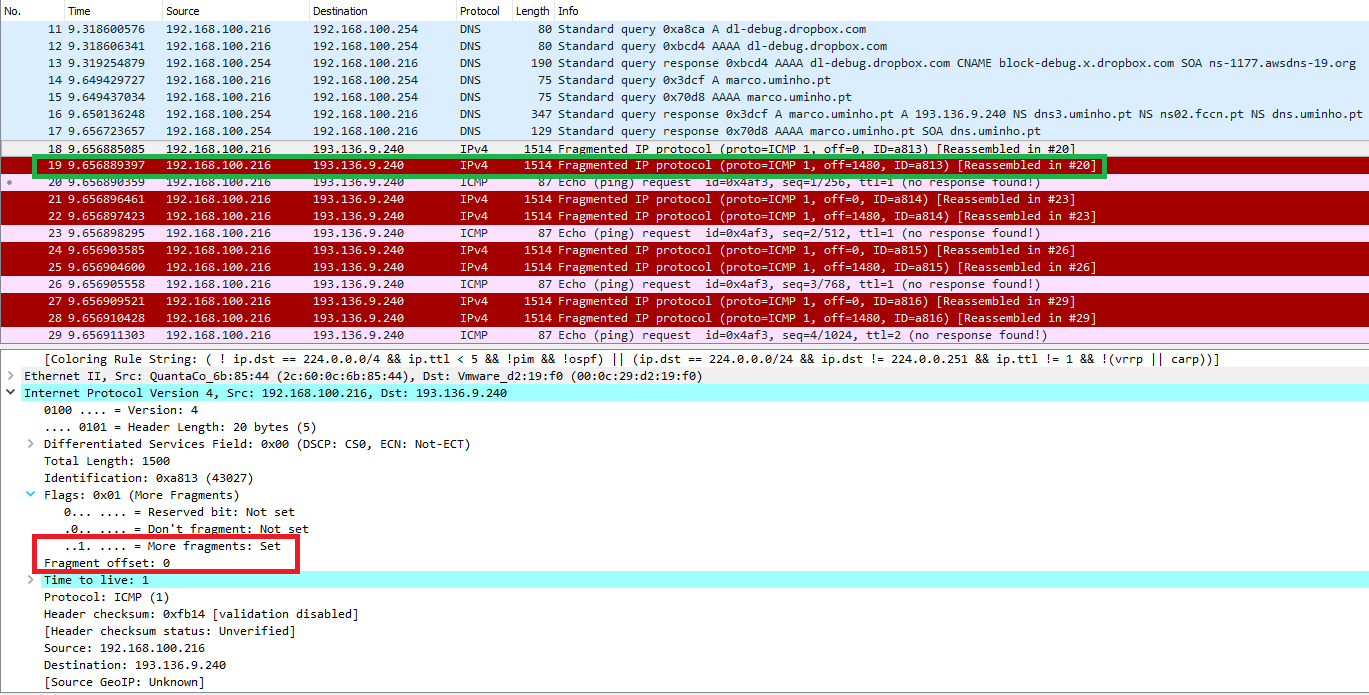
\includegraphics[scale=0.35]{./imagens/packet_first.png} 
	\end{center}
	\caption{\label{fig:packet_first}As flags e o fragment offset confirmam que é o primeiro fragmento.}
\end{figure} 

\subsection{Exercício 3.c.}
\subsubsection{Questão}\rule[-10pt]{0pt}{10pt}\\

Imprima o segundo fragmento do datagrama IP original. Que informação do cabeçalho IP indica que não se trata do 1º fragmento? Há mais fragmentos? O que nos permite afirmar isso?

\subsubsection{Resposta}\rule[-10pt]{0pt}{10pt}\\

Sabe-se que este não é o primeiro segmento pois o datagrama em questão tem \textit{fragment offset} = 1480. Isto significa que, no datagrama original, este segmento começará a partir do byte 1480 do datagrama. Analisando a \textit{flag more fragments}, percebe-se existem mais fragmentos, visto que esta é igual a 1.

\subsubsection{Realização}\rule[-10pt]{0pt}{10pt}\\

\begin{figure}
	\begin{center}
	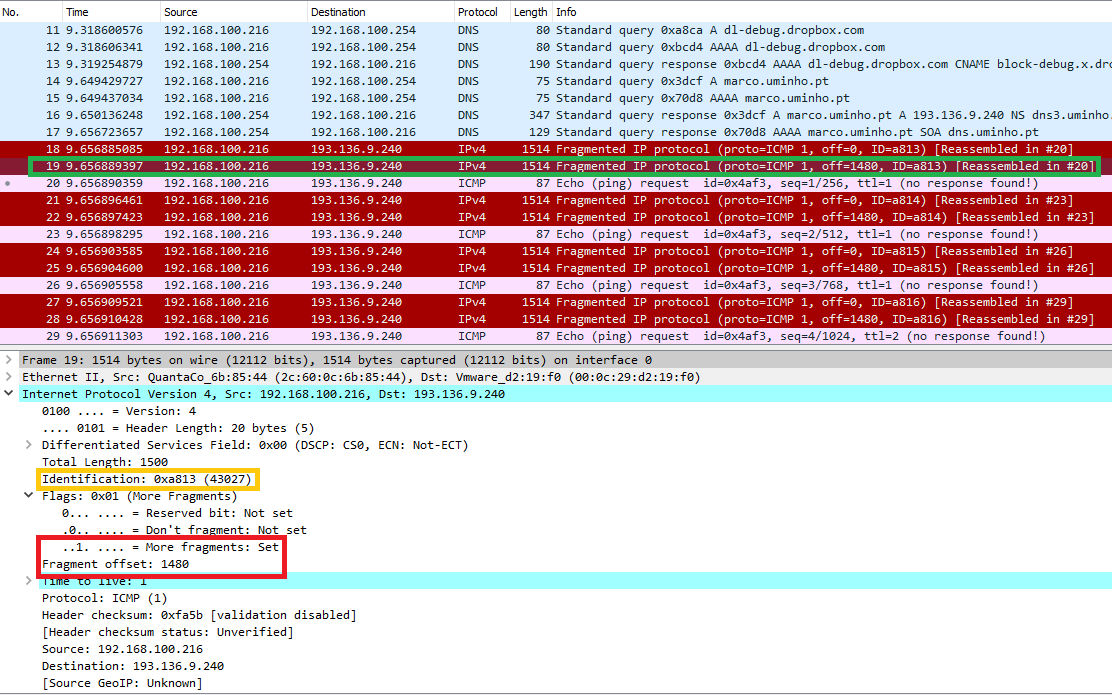
\includegraphics[scale=0.35]{./imagens/packet_second.png} 
	\end{center}
	\caption{\label{fig:packet_second}As flags e o fragment offset confirmam que é o segundo fragmento.}
\end{figure} 

\subsection{Exercício 3.d.}
\subsubsection{Questão}\rule[-10pt]{0pt}{10pt}\\

Quantos fragmentos foram criados a partir do datagrama original? Como se detecta o último fragmento correspondente ao datagrama original?

\subsubsection{Resposta}\rule[-10pt]{0pt}{10pt}\\

Analisando o parâmetro \textit{identification} dos datagramas capturados pelo \textit{Wireshark}, percebe-se que existem três datagramas com o mesmo valor o que revela que pertencem ao mesmo PDU (\textit{identification} = 0xa813). Desta forma podemos concluir que o datagrama foi fragmentado duas vezes resultando em três fragmentos.
	
A deteção do último fragmento é feita através da análise da \textit{flag more fragments}. Se esta estiver a 1 então existem mais segmentos. Caso contrário, o segmento em questão é o último.

\subsubsection{Realização}\rule[-10pt]{0pt}{10pt}\\

\begin{figure}[h]
	\centering
	\begin{subfigure}{.4\textwidth}
		\centering
		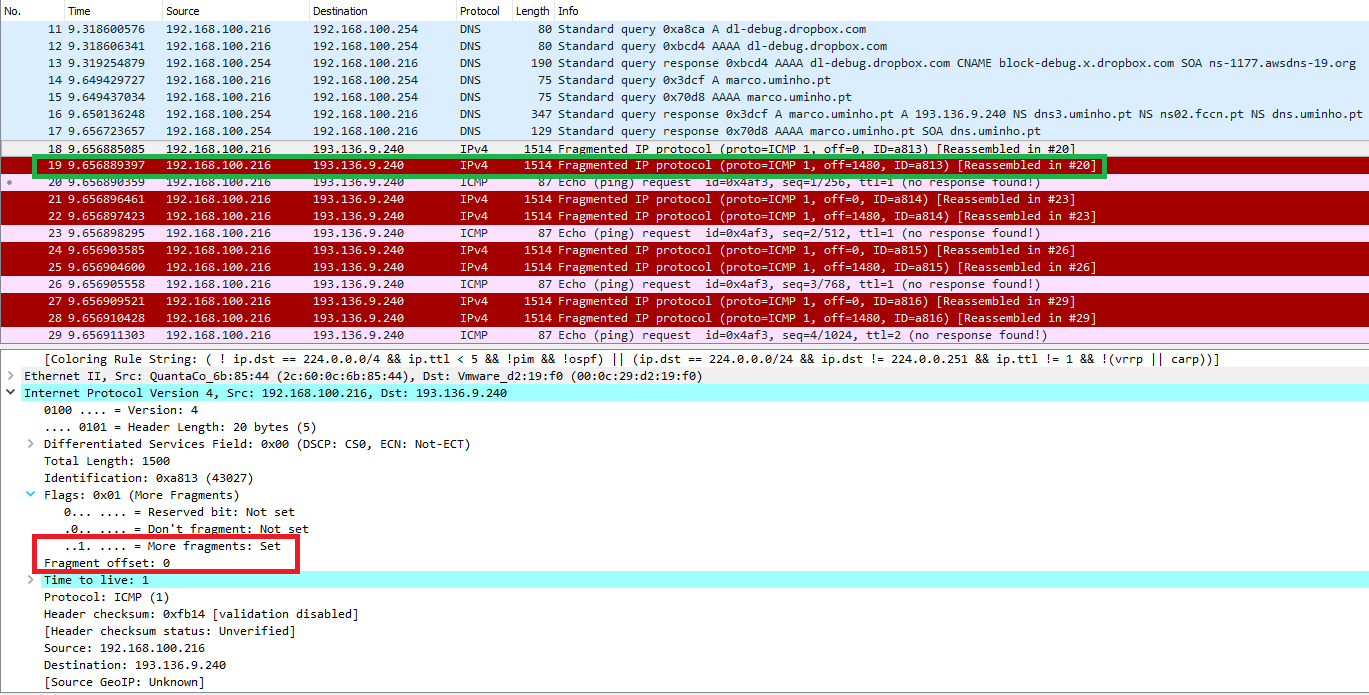
\includegraphics[width=0.98\linewidth]{./imagens/packet_first.png}
	\end{subfigure}%
	\begin{subfigure}{.4\textwidth}
		\centering
		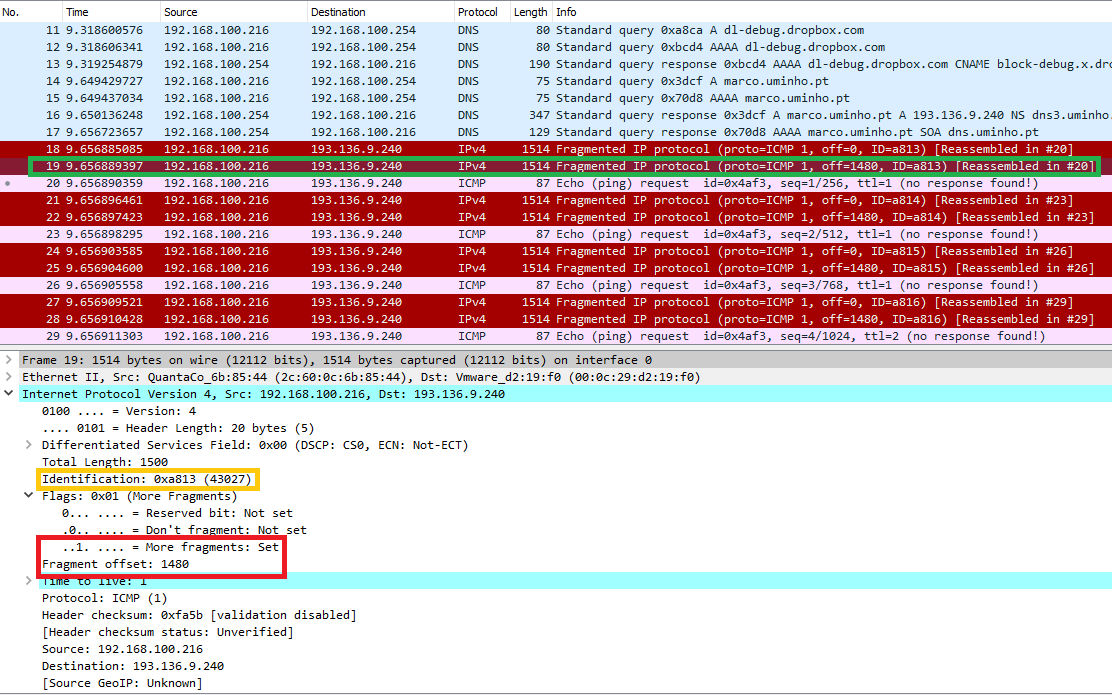
\includegraphics[width=0.98\linewidth]{./imagens/packet_second.png}
	\end{subfigure}%
	\begin{subfigure}{.4\textwidth}
		\centering
		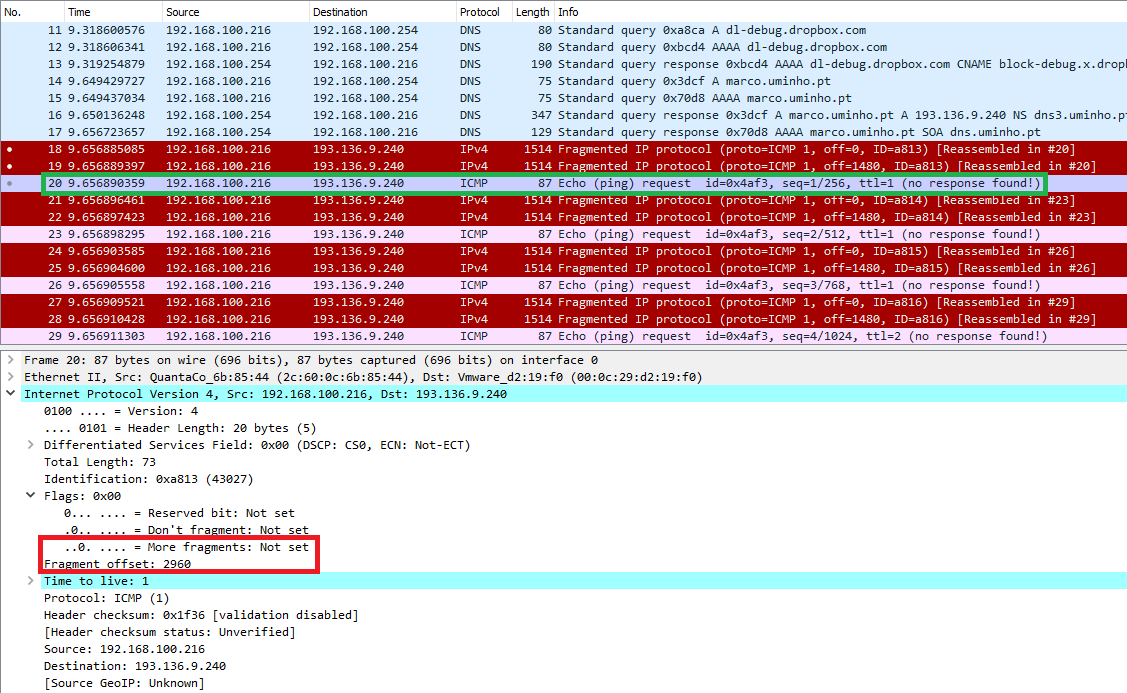
\includegraphics[width=0.98\linewidth]{./imagens/packet_third.png}
	\end{subfigure}
	\caption{Encontrando vários fragmentos com a mesma \textit{identification}, é possível saber a sua ordem através do \textit{fragment offset} e flags.}
	\label{fig:field_packet}
\end{figure}

\subsection{Exercício 3.e.}
\subsubsection{Questão}\rule[-10pt]{0pt}{10pt}\\

Indique, resumindo, os campos que mudam no cabeçalho IP entre os diferentes fragmentos, e explique a forma como essa informação permite reconstruir o datagrama original. 

\subsubsection{Resposta}\rule[-10pt]{0pt}{10pt}\\

Os campos que mudam são \textit{Total Length, more fragments} e \textit{Fragment offset}. 

No primeiro fragmento, o \textit{Total Length} é igual ao MTU menos o \textit{Header Length}, a flag \textit{more fragments} é igual a 1 e o \textit{Fragment offset} é igual a 0.

Entre o primeiro fragmento e o último fragmento não inclusives, o \textit{Total Length} é igual ao MTU menos o \textit{Header Length}, a flag \textit{more fragments} é igual a 1 e o \textit{Fragment offset} é igual a (MTU - \textit{Header Length}) * (n - 1), n sendo o n-ésimo fragmento do datagrama (n = 1, 2, ...).

No último fragmento, o \textit{Total Length} é menor ou igual ao MTU, a flag \textit{more fragments} é igual a 0 e o \textit{Fragment offset} é igual a (MTU - \textit{Header Length}) * (n - 1), n sendo o número de fragmentos do datagrama.

\subsubsection{Realização}\rule[-10pt]{0pt}{10pt}\\
Verifica-se no datagrama analisado que as \textit{flags} e o \textit{fragment offset} evoluem como indicado.
~\ref{fig:field_packet} 


\pagebreak
\section{Parte II - Endereçamento e Encaminhamento IP}

\subsection{Exercício 2.1.a}
\subsubsection{Questão}\rule[-10pt]{0pt}{10pt}\\

Indique que endereços IP e máscaras de rede foram atribuídos pelo CORE a cada equipamento. Para simplificar, pode incluir uma imagem que ilustre de forma clara a topologia definida e o endereçamento usado.

\subsubsection{Resposta}\rule[-10pt]{0pt}{10pt}\\

A máscara de rede utilizada é 255.255.255.0. Isto deve-se a facto de todos os IPv4 atribuídos aos diferentes componentes da rede terem /24 como quantidade de bits que identificam a rede.

\begin{figure}
	\begin{center}
	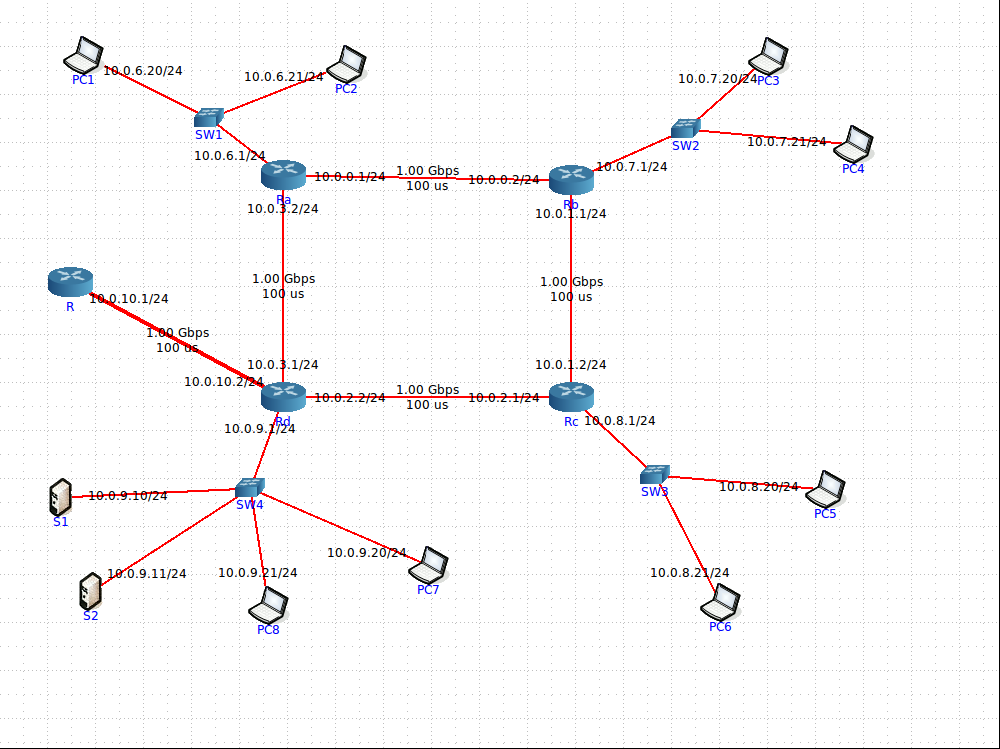
\includegraphics[scale=0.35]{./imagens/rede.png} 
	\end{center}
	\caption{\label{fig:rede}Topologia da rede.}
\end{figure} 

\subsection{Exercício 2.1.b}
\subsubsection{Questão}\rule[-10pt]{0pt}{10pt}\\

Tratam-se de endereços públicos ou privados? Porquê?

\subsubsection{Resposta}\rule[-10pt]{0pt}{10pt}\\

Tratam-se de endereços privados pois o primeiro octeto é 00001010, que em decimal representa 10. Sendo este o primeiro octeto podemos afirmar que é um endereço IP privado visto que pertence ao conjunto de prefixos que identificam um endereçamento privado. Os conjuntos de endereços privados são os seguintes: 

\begin{itemize}
	\item Start address: 10.0.0.0 $\,\to\,$ End Address: 10.255.255.255
	\item Start address: 172.16.0.0 $\,\to\,$ End Address: 172.31.255.255
	\item Start address: 192.168.0.0 $\,\to\,$ End Address: 192.168.255.255
	\item Start address: 169.254.0.0 $\,\to\,$ End Address: 169.254.255.255
\end{itemize}

\subsubsection{Realização}\rule[-10pt]{0pt}{10pt}\\

Pela observação da topologia da rede ~\ref{fig:rede}.

\subsection{Exercício 2.1.c}
\subsubsection{Questão}\rule[-10pt]{0pt}{10pt}\\

Porque razão não é atribuído um endereço IP aos switches?

\subsubsection{Resposta}\rule[-10pt]{0pt}{10pt}\\

Na topologia em questão se vier um pacote com destino ao PC7, este vem com endereço de destino de 10.0.9.20/24. Para tal, o pacote vem do \textit{router} R e chega ao \textit{router} Rd. O \textit{router} Rd aplica a NetMask 255.255.255.0 ao endereço de destino e obtém 10.0.9.0. Consegue fazer match no endereço 10.0.9.1 e envia o pacote para o SW4. Ao chegar ao SW4, este avalia o endereço MAC de destino e duas situações podem acontecer. Se este tiver nos seus registos o endereço, então envia diretamente ao host especificado. Caso não tenha ainda essa informação envia para todos os hosts a ele ligados.

Efetivamente, os \textit{switches} não operam ao nível de rede e como tal a camada de rede, nomeadamente o IP, é completamente transparente para estes dispositivos.

Através do exemplo a cima podemos concluir que não é necessário que este tenha IP pois os pacotes são enviados para o \textit{switch} com base no IP da interface de saída do \textit{router}. Após o datagrama chegar ao \textit{switch} este quanto muito usa endereços MAC por forma a fazer \textit{forward} do datagrama para o \textit{host} respetivo.

\subsection{Exercício 2.1.d}
\subsubsection{Questão}\rule[-10pt]{0pt}{10pt}\\

Usando o comando ping certifique-se que existe conectividade IP entre os laptops dos vários departamentos e os servidores do departamento D (basta certificar-se da conectividade de um laptop por departamento).

\pagebreak
\subsubsection{Resposta}\rule[-10pt]{0pt}{10pt}\\

\begin{figure}[h]
	\centering
	\begin{subfigure}{.5\textwidth}
		\centering
		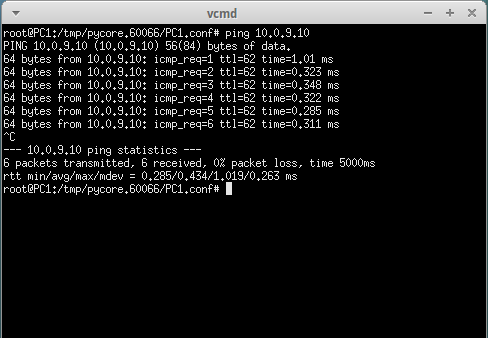
\includegraphics[width=0.75\linewidth]{./imagens/PC1_S1.png}
	\end{subfigure}%
	\begin{subfigure}{.5\textwidth}
		\centering
		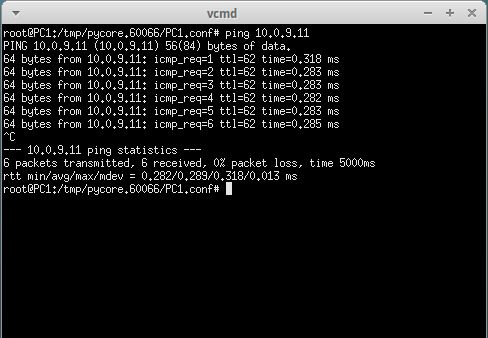
\includegraphics[width=0.75\linewidth]{./imagens/PC1_S2.png}
	\end{subfigure}
	\caption{Teste de conectividade entre PC1 e os servidores S1 (à esquerda) e S2 (à direita).}
	\label{fig:pc1_s}
\end{figure}

\begin{figure}[h]
	\centering
	\begin{subfigure}{.5\textwidth}
		\centering
		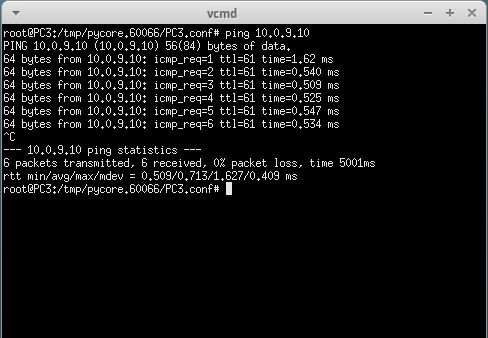
\includegraphics[width=0.75\linewidth]{./imagens/PC3_S1.png}
	\end{subfigure}%
	\begin{subfigure}{.5\textwidth}
		\centering
		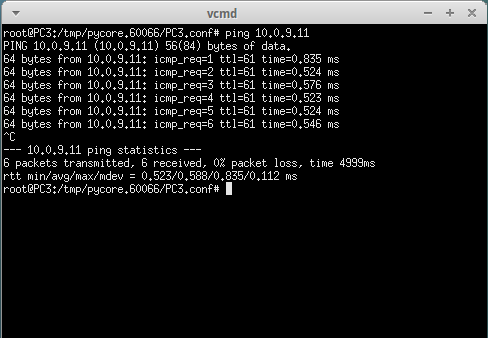
\includegraphics[width=0.75\linewidth]{./imagens/PC3_S2.png}
	\end{subfigure}
	\caption{Teste de conectividade entre PC3 e os servidores S1 (à esquerda) e S2 (à direita).}
	\label{fig:pc3_s}
\end{figure}

\begin{figure}[h]
	\centering
	\begin{subfigure}{.5\textwidth}
		\centering
		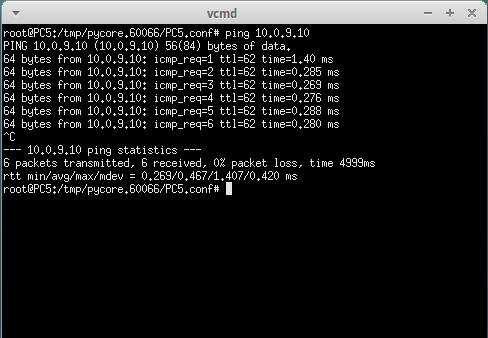
\includegraphics[width=0.75\linewidth]{./imagens/PC5_S1.png}
	\end{subfigure}%
	\begin{subfigure}{.5\textwidth}
		\centering
		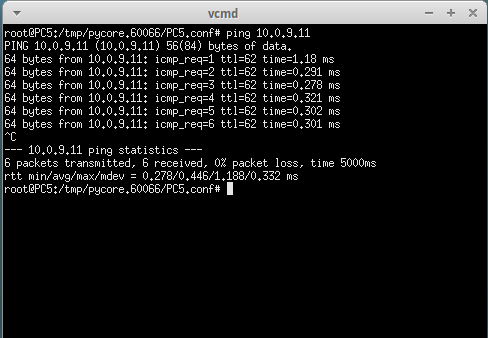
\includegraphics[width=0.75\linewidth]{./imagens/PC5_S2.png}
	\end{subfigure}
	\caption{Teste de conectividade entre PC5 e os servidores S1 (à esquerda) e S2 (à direita).}
	\label{fig:pc5_s}
\end{figure}

\begin{figure}[h]
	\centering
	\begin{subfigure}{.5\textwidth}
		\centering
		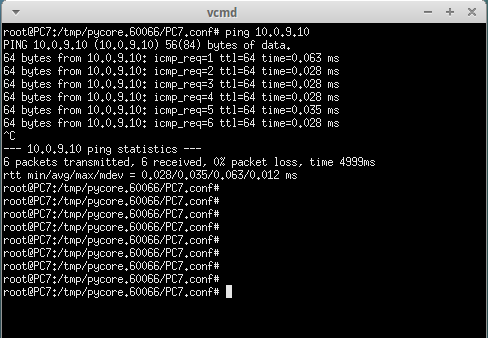
\includegraphics[width=0.75\linewidth]{./imagens/PC7_S1.png}
	\end{subfigure}%
	\begin{subfigure}{.5\textwidth}
		\centering
		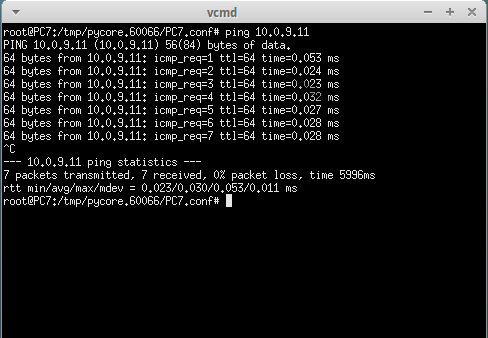
\includegraphics[width=0.75\linewidth]{./imagens/PC7_S2.png}
	\end{subfigure}
	\caption{Teste de conectividade entre PC7 e os servidores S1 (à esquerda) e S2 (à direita).}
	\label{fig:pc7_s}
\end{figure}

Tendo em conta os resultados do comando \textit{ping} pode-se afirmar que existe conetividade entre os \textit{hosts} dos diferentes departamentos e os servidores do departamento D.

\subsection{Exercício 2.1.e}
\subsubsection{Questão}\rule[-10pt]{0pt}{10pt}\\

Verifique se existe conectividade IP do router de acesso para os servidores S1 e S2.

\subsubsection{Resposta}\rule[-10pt]{0pt}{10pt}\\

\begin{figure}[h]
	\centering
	\begin{subfigure}{.5\textwidth}
		\centering
		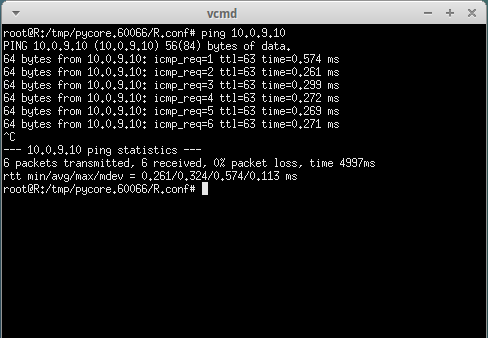
\includegraphics[width=0.75\linewidth]{./imagens/R_S1.png}
	\end{subfigure}%
	\begin{subfigure}{.5\textwidth}
		\centering
		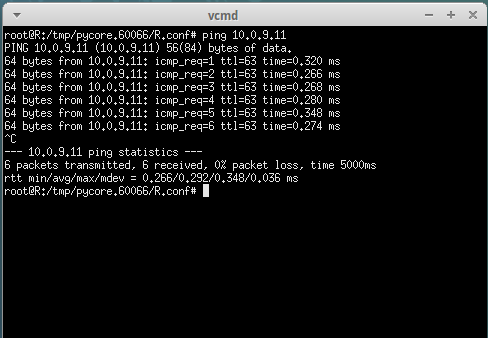
\includegraphics[width=0.75\linewidth]{./imagens/R_S2.png}
	\end{subfigure}
	\caption{Teste de conectividade entre R e os servidores S1 (à esquerda) e S2 (à direita).}
	\label{fig:r_s}
\end{figure}

Tendo em conta os resultados obtidos em ~\ref{fig:r_s}, podemos afirmar que exite conetividade entre o \textit{router} R e os servidores S1 e S2.


% Exercicio 2 --------------------

\subsection{Exercício 2.2.a}
\subsubsection{Questão}\rule[-10pt]{0pt}{10pt}\\

Execute o comando netstat ¿rn por forma a poder consultar a tabela de encaminhamento unicast (IPv4). Inclua no seu relatório as tabelas de encaminhamento obtidas; interprete as várias entradas de cada tabela. Se necessário, consulte o manual respetivo ( man netstat ).

\subsubsection{Resposta}\rule[-10pt]{0pt}{10pt}\\

A primeira linha na tabela de endereçamento do PC3 representa a rota por defeito, isto é, quando entre no PC3 um datagrama com um IP que não faz \textit{match} com nenhum IP da coluna \textit{Destination} então este é reencaminhado para o \textit{router} de acesso, ou seja, 10.0.7.1 ficando este responsável pelo seu encaminhamento. Denotando que a primeira linha, por ser um endereço estático, tem a menor prioridade. Esta linha faz \textit{match} com qualquer endereço pois tem uma \textit{Genmask} igual a 0.0.0.0. Efetivamente, quando chega à máquina PC3, por exemplo,  um datagrama com o IP 10.0.8.20, este é comparado com todas as linhas da tabela. Posteriormente é aplicada a máscara obtendo-se 0.0.0.0. O resultado é depois comparado com o campo \textit{Destination} e faz match. De seguida é enviado para o router de acesso explicitado pelo campo \textit{Gateway}

A segunda linha é responsável por encaminhar, através da própria máquina, o trânsito local, ou seja, o prórprio PC3 encaminha os datagramas para \textit{hosts} vizinhos. Deste modo, todos os datagramas que tiverem como prefixo de rede 10.0.7 vão fazer match na segunda linha, isto porque, chegando por exemplo o datagrama com o IP 10.0.7.21, é aplicada a máscara 255.255.255.0 e resulta a \textit{destination} 10.0.7.0. Posteriormente é enviado para o endereço dito no \textit{Gateway}, 0.0.0.0, ou seja, fica responsável por encaminhar este datagrama a própria máquina. Este processo de encaminhamento resulta pois os \textit{hosts} tem conhecimento da topologia da rede local.

A tabela de encaminhamento do \textit{router} Rb não incluí rotas por defeito pois todas as rotas existentes na rede encontram-se identificadas na tabela à partida.

Através da análise da topologia na rede criada com o CORE percebemos que o \textit{router} Rb deverá ser responsável por encaminhar para a rede 10.0.0.0, 10.0.1.0, e 10.0.7.0. A tabela de encaminhamento confirma as nossas suspeitas, pois todas as linhas que têm os endereços IP atrás indicados têm como \textit{Gateway} 0.0.0.0, que significa que o próprio \textit{router} fica responsável por encaminhar esses datagramas.

Todas as outras redes existentes encontram-se na tabela com o endereço de encaminhamento apropriado. Nomeadamente, caso os datagramas tenham como destino a rede 10.0.x.0, em que x={2,3,6,8,9,10}, estes são reencaminhados para uma das duas redes a que o \textit{router} Rb tem acesso, isto é, 10.0.0.1 ou 10.0.1.2. Estas entradas em espicífico na tabela têm a \textit{flag} G no campo \textit{Flags}, visto não ser um encaminhamento direto.

\subsubsection{Realização}\rule[-10pt]{0pt}{10pt}\\

\begin{figure}[h]
	\centering
	\begin{subfigure}{.5\textwidth}
		\centering
		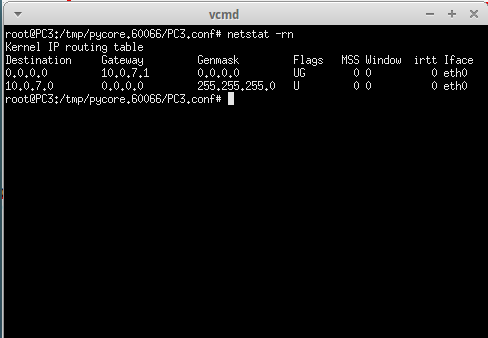
\includegraphics[width=0.95\linewidth]{./imagens/netstatPC3.png}
	\end{subfigure}
	\begin{subfigure}{.5\textwidth}
		\centering
		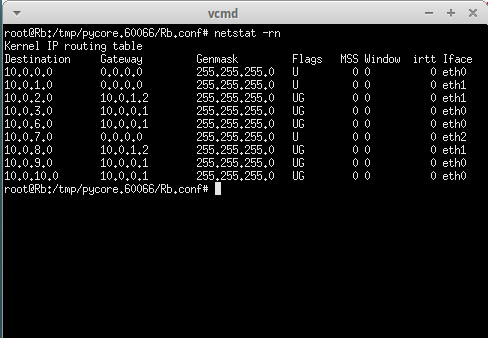
\includegraphics[width=0.95\linewidth]{./imagens/netstatRb.png}
	\end{subfigure}
	\caption{Tabelas de encaminhamento do PC3 (à esquerda) e do Rb (à direita).}
	\label{fig:r_s}
\end{figure}

\subsection{Exercício 2.2.b}
\subsubsection{Questão}\rule[-10pt]{0pt}{10pt}\\
\subsubsection{Resposta}\rule[-10pt]{0pt}{10pt}\\
\subsubsection{Realização}\rule[-10pt]{0pt}{10pt}\\

\subsection{Exercício 2.2.c}
\subsubsection{Questão}\rule[-10pt]{0pt}{10pt}\\
\subsubsection{Resposta}\rule[-10pt]{0pt}{10pt}\\
\subsubsection{Realização}\rule[-10pt]{0pt}{10pt}\\

\subsection{Exercício 2.2.d}
\subsubsection{Questão}\rule[-10pt]{0pt}{10pt}\\
\subsubsection{Resposta}\rule[-10pt]{0pt}{10pt}\\
\subsubsection{Realização}\rule[-10pt]{0pt}{10pt}\\

\subsection{Exercício 2.2.e}
\subsubsection{Questão}\rule[-10pt]{0pt}{10pt}\\
\subsubsection{Resposta}\rule[-10pt]{0pt}{10pt}\\
\subsubsection{Realização}\rule[-10pt]{0pt}{10pt}\\

% Exercicio 3 --------------------

\subsection{Exercício 3.1}
\subsubsection{Questão}\rule[-10pt]{0pt}{10pt}\\

Considere que dispõe apenas do endereço de rede IP 172.16.0.0/16, defina um novo esquema de endereçamento para as redes dos departamentos (mantendo a rede de acesso e core inalteradas) e atribua endereços às interfaces dos vários sistemas envolvidos. Deve justificar as opções usadas.

\subsubsection{Resposta}\rule[-10pt]{0pt}{10pt}\\


\par A partir do endereço dado, decidiu-se criar um conjunto de subredes de endereço 172.16.0.0/24, dando 8 bits para criação de subredes e 8 bits para criação de \textit{hosts} dentro de cada subrede, de modo a maximizar a flexibilidade da rede para instalações futuras. Prosseguimos então à redefenição do esquema de endereçamento:
\begin{itemize}
\item \textbf{Ra}: Definimos o IP como 172.16.1.1/24 na interface eth2 (ligação ao Departamento A). A escolha do terceiro octeto a 1 reside no facto de este ter sido a primeira subrede a ser endereçada e 1 no quarto octeto reside no facto de ser o primeiro dispositivo/host da subrede. Propagou-se então os endereços da subnetting para os PC's do departamento. No caso do PC1 recebeu o endereço IP 172.16.1.2/24 e o PC2 recebeu o endereço IP 172.16.1.3/24.

\item \textbf{Rb}: Repetiu-se o processo mas com 172.16.2.1/24 para a interface eth2 do router (ligação ao Departamento B). A escolha do terceiro octeto a 2 reside no facto de este ter sido a segunda subrede a ser endereçada. Propagou-se o IP da subnetting para os PC3 e PC4 com os IP 172.16.2.2/24 e 172.16.2.3/24, respetivamente.

\item \textbf{Rc}: Repetiu-se o processo mas com 172.16.3.1/24 para a interface eth2 do router (ligação ao Departamento C). A escolha do terceiro octeto a 3 reside no facto de este ter sido a terceira subrede a ser endereçada. Propagou-se o IP da subnetting para os PC5 e PC6 com os IP 172.16.3.2/24 e 172.16.3.3/24, respetivamente.

\item \textbf{Rd}: Repetiu-se o processo mas com 172.16.4.1/24 para a interface eth4 do router (ligação ao Departamento D). A escolha do terceiro octeto a 4 reside no facto de este ter sido a quarta subrede a ser endereçada. Propagou-se para PC7, PC8, S1 e S2 172.16.4.2/24, 172.16.4.3/24, 172.16.4.4/24 e 172.16.4.5/24, respetivamente.

\end{itemize}

\subsubsection{Realização}\rule[-10pt]{0pt}{10pt}\\

\begin{figure}
	\begin{center}
	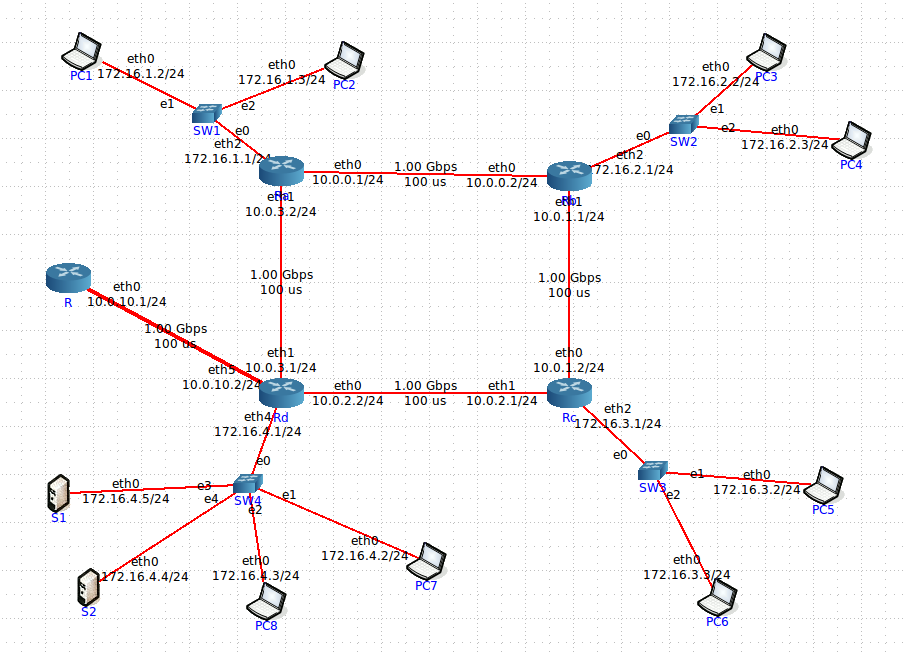
\includegraphics[scale=0.35]{./imagens/redeIPSnovos.png} 
	\end{center}
	\caption{\label{fig:ping}As subredes mantêm a capacidade de enviar pacotes entre si.}
\end{figure} 


\subsection{Exercício 3.2}
\subsubsection{Questão}\rule[-10pt]{0pt}{10pt}\\

Qual a máscara de rede que usou (em formato decimal)? Quantos hosts IP pode interligar em cada departamento? Justifique.

\subsubsection{Resposta}\rule[-10pt]{0pt}{10pt}\\

A máscara da rede IP é 255.255.0.0 , sendo a máscara para cada subrede 255.255.255.0 . Isto permite-nos 8 bits para endereçar os \textit{hosts} de cada departamento. Como os \textit{hosts} 172.16.x.0/24 e 172.16.x.255/24 estão reservados como o identificador da subrede e acesso de \textit{broadcast}, respetivamente, dispomos de 2\^{}8 - 2 = 254 \textit{hosts} por departamento. 



\subsection{Exercício 3.3}
\subsubsection{Questão}\rule[-10pt]{0pt}{10pt}\\

Garanta e verifique que conectividade IP entre as várias redes locais da organização MIEI-RC é mantida.

\subsubsection{Resposta}\rule[-10pt]{0pt}{10pt}\\

Recorrendo ao comando \textit{ping}, verificou-se que a conetividade IP das subredes da organização e confirmou-se que cada subrede se pode ligar a cada uma das outras subredes locais.

\subsubsection{Realização}\rule[-10pt]{0pt}{10pt}\\ 


\begin{figure}
	\begin{center}
	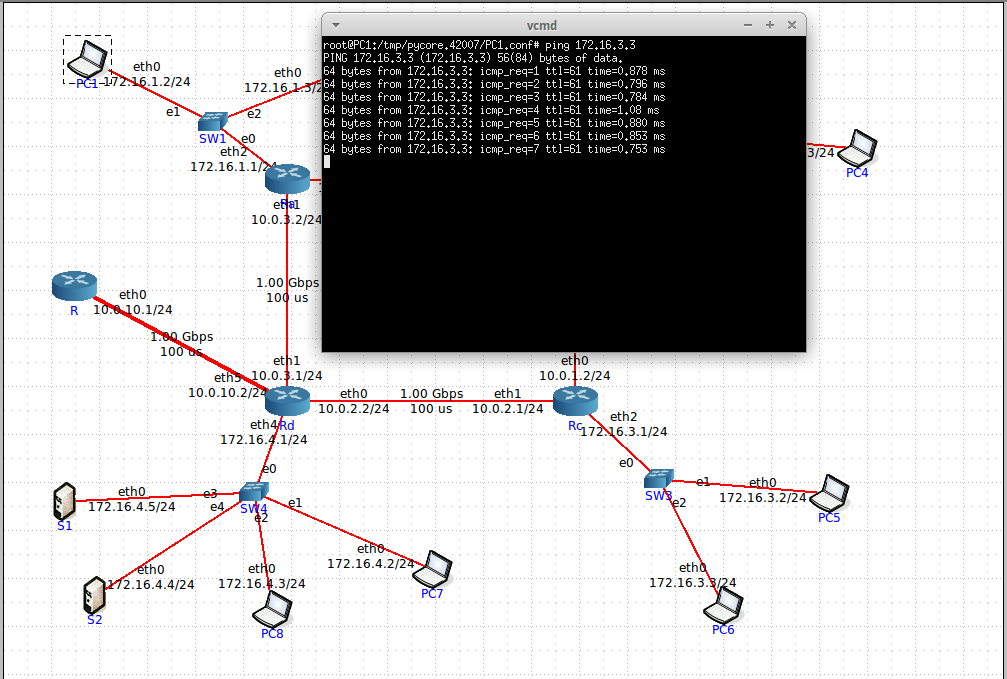
\includegraphics[scale=0.35]{./imagens/exercicio3_3.png} 
	\end{center}
	\caption{\label{fig:ping}As subredes mantêm a capacidade de enviar pacotes entre si.}
\end{figure} 



\section{Conclusions}
Neste trabalho...

%BIBLIOGRAFIA
\bibliographystyle{splncs}
\bibliography{ficheirodebibliografia}

\end{document}
